\chapter{Exercises}
\subsubsection{Ex 1}
Since metric is \[
ds^{2}= dx^{2} +dy^{2}
\]
then metric tensor in this coordinates system is
\[
\begin{pmatrix}
1 & 0 \\
0 & 1
\end{pmatrix} 
\]
Now, requested transformation rule for (0,2) tensor is
\[
g_{\mu ^{\prime }\nu ^{\prime }} = \frac{d x^{\mu }}{d x^{\mu ^{\prime }}} \frac{d x^{\nu }}{d x^{\nu ^{\prime }}} g_{\mu \nu }
\]
those partial derivatives are the Jacobian, to compute it I have to express old coordinates in function of new coordinates:
\[
\begin{cases}
u = \left( x+y \right)/2 \\
v = \left( x-y \right)/2 \\
\end{cases} \to 
\begin{cases}
x = u+v \\
y = u-v \\
\end{cases}
\]
then the Jacobian is 
\[
\frac{d x^{\mu }}{d x^{\mu ^{\prime }}} = \begin{pmatrix}
dx^{0}/dx^{0^{\prime }} & dx^{0}/dx^{1^{\prime }} \\
dx^{1}/dx^{0^{\prime }} & dx^{1}/dx^{1^{\prime }}
\end{pmatrix} = \begin{pmatrix}
1 & 1 \\
1 & -1
\end{pmatrix} 
\]
with $x^{0}=x, x^{1} = y$, I apply transformation rule, just for first term, other follows straight up
\[
g_{0^{\prime }0^{\prime }} = \frac{d x^{\mu }}{d x^{0^{\prime }}}\frac{d x^{\nu }}{d x^{0^{\prime }}} g_{\mu \nu } = \frac{d x^{0}}{d x^{0^{\prime }}}\frac{d x^{0}}{d x^{0^{\prime }}} g_{00} + \frac{d x^{1}}{d x^{0^{\prime }}}\frac{d x^{1}}{d x^{0^{\prime }}} g_{11} = \left( 1\cdot1\cdot1 \right) + \left( 1\cdot1\cdot1 \right) = 2
\]
other terms of the metric tensor $g_{\mu \nu }$ are omitted since they're null. 
\[
g_{\mu ^{\prime }\nu ^{\prime }} = \begin{pmatrix}
2 & 0 \\
0 & 2
\end{pmatrix} 
\]

\subsubsection{Ex 2}

\[
ds^{2} = dr^{2}+r^{2}d\phi ^{2}
\]
First question: how many free Christoffel symbols?
\[
\Gamma ^{\mu \to 2}_{\nu \rho \to 2\cdot 2 = 4}, 	
\]
8 total, since symmetry on lower two, we have $4 \to  3$, then $2\cdot3=6$.\par
Second quesstion: how many Christoffel symbols do not vanish?\par
\begin{gather*}
g_{\mu \nu } = \begin{pmatrix}
1 & 0 \\
0 & r^{2}
\end{pmatrix} ; g^{\mu \nu } = \frac{1}{r^{2}} \begin{pmatrix}
r^{2} & 0 \\
0 & 1
\end{pmatrix}  = \begin{pmatrix}
1 & 0 \\
0 & \frac{1}{r^{2}}
\end{pmatrix} 
\end{gather*}
with this you can determine how many non vanishing Christoffel symbols there are.
\[
\Gamma ^{\sigma }_{\mu \nu } = \frac{1}{2} G^{\sigma \rho }\left( \partial_{\mu }g_{\nu \rho }+\partial_{\nu }g_{\rho \mu }-\partial_{\rho }g_{\mu \nu } \right)
\]
we see that only non-zero component of derivative of metric is $\partial_{r}g_{\phi \phi } = 2r$, and only non-zero component of inverse metric are $g_{\rho \sigma }, \rho =\sigma $.
\begin{gather*}
\Gamma ^{x}_{xx} = \oslash \\
\Gamma ^{r}_{r\phi } = \Gamma ^{r}_{\phi r} = \oslash\\
\Gamma ^{r}_{\phi \phi } = \frac{1}{2}g^{rr}\left( \partial_{\phi }g_{\phi r} + \partial_{\phi }g_{r\phi }-\partial_{r}g_{\phi \phi } \right) = -\frac{1}{2}\cdot 2r = -r\\
\Gamma ^{\phi }_{rr } = \oslash\\
\Gamma ^{\phi }_{r\phi } = \Gamma ^{\phi }_{\phi r} = \frac{1}{2}g_{\phi \phi } \left( \partial_{\phi }g_{r\phi } + \partial_{r}g_{\phi \phi }-\partial_{\phi }g_{\phi r} \right) = \frac{1}{2}\cdot 2r\cdot \frac{1}{r^{2}}\\
\Gamma ^{\phi }_{\phi \phi } = \oslash
\end{gather*}

\subsubsection{Ex 3}
Same as Ex 2
\subsubsection{Ex 4}
Same as Ex 2,3
\subsubsection{Ex 5}
\[
ds^{2} = -\left( 1+2\phi  \right)dt^{2} +\left( 1-2\phi  \right)dr^{2}+r^{2}d\theta ^{2}+r^{2}\text{sin}^{2}\theta d\phi ^{2}, \phi = - \frac{GM}{r}	
\]
To compute time, I need to compute an interval, but since both clock stand still in their position, in any generic interval, spatial coordinates vanish. I'm left with
\[
ds^{2} = -\left( 1+2\phi  \right)dt^{2}
\]
Being $d\tau ^{2} =- ds^{2} = \left( 1+2\phi  \right)dt^{2}$,
\[
	d\tau  = \sqrt{1+2\phi }dt
\]
After integrating in \emph{dt} in interval $\left[ 0,t \right]$:
\begin{gather*}
	\tau _{1} = \sqrt{1+2\phi \left( R \right)}t \\
	\tau _{2} = \sqrt{1+2\phi \left( R+h \right)}t
\end{gather*}

\begin{gather*}
	\frac{\tau _{2}}{\tau _{1}} = \frac{\sqrt{1+2\phi\left( R+h \right)}}{\sqrt{1+2\phi \left( R \right)}} \\
\phi \left( R+h \right) = \phi \left( R \right) +\phi ^{\prime }\left( R \right)h +\ldots = - \frac{GM}{R} + \frac{GMh}{R^{2}} +\ldots 	 
\end{gather*}

\begin{gather*}
\frac{\tau _{2}}{\tau _{1}} = \frac{\sqrt{1+2\phi \left( R+h \right)}}{\sqrt{1+2\phi \left( R \right)}} = \frac{\sqrt{1-2\phi \left( R \right) +2\phi^{\prime } \left( R \right)h }}{\sqrt{1-2\phi \left( R \right)}} = \sqrt{1 + \frac{ 2\phi^{\prime }\left( R \right)h}{1 -2\phi \left( R \right)}}
\end{gather*}
Then you do some simplifications and then do series expansion for $\sqrt{1+x} \approx 1 + \frac{x}{2}$, and you should get 
\[
\frac{\Delta \tau _{2}}{\Delta \tau _{1}} \approx 1 + \frac{GMh}{2R\left( R-2GM \right)}
\]

\subsubsection{Ex 6}

If you don't remember, you can get the geodesics equation from
\[
\frac{D}{d\lambda }\left( \frac{dx^{\nu }}{d\lambda } \right) = \frac{d x^{\mu }}{d \lambda }\nabla _{\mu }\left( \frac{d x^{\nu }}{d \lambda } \right) = \ldots 
\]
So we get two geodesics equations:
\begin{gather}
	\frac{d ^{2}x^{\phi }}{d \lambda ^{2}} + \Gamma ^{\phi }_{\theta \phi }\frac{d x^{\theta }}{d \lambda }\frac{d x^{\phi }}{d \lambda } =0  = \frac{d ^{2}x^{\phi }}{d \lambda ^{2}} + \frac{\text{cos}\theta }{\text{sin}\theta }\frac{d x^{\theta }}{d \lambda }\frac{d x^{\phi }}{d \lambda } \label{ex:1g}\\
	\frac{d^{2}x^{\theta }}{d\lambda ^{2}} + \Gamma ^{\theta }_{\phi \phi }\frac{d x^{\phi }}{d \lambda }\frac{d x^{\phi }}{d \lambda } = 0  = \frac{d ^{2}\theta }{d \lambda ^{2}} - \text{sin}\theta \text{cos}\theta \frac{d x^{\phi }}{d \lambda }\frac{d x^{\phi }}{d \lambda }\label{ex:2g}
\end{gather}
Now you have to check both conditions for both equations.\par
First one: constant longitude means $\frac{d x^{\phi }}{d \lambda } = 0$, I think it's trivial. \par
Second one: you get that in \ref{ex:1g}, since we are at constant latitude, vanishes. In \ref{ex:2g} you get that the second term vanishes only for $\theta =0 , \frac{\pi }{2}$, but only 0 is a geodesics, other solution are the poles, degenerate solution. 

\subsubsection{Ex 7}
First request, just compute everything. Be aware to use all combinations.\par
Second request: use product rule so
\begin{align*}
	\nabla _{\mu }\left( V^{\nu }V^{\nu } \right) &= \partial_{\mu }\left( V^{\nu }V_{\nu } \right)\\
	\left( \nabla _{\mu }V^{\nu } \right)V_{\nu } + V^{\nu }\left( \nabla _{\mu }V_{\nu } \right) &= \left( \partial_{\mu }V^{\mu } \right)V_{\nu } + V^{\nu }\left( \partial_{\mu }V_{\nu } \right)
\end{align*}
Then you compute the covariant derivatives, you will find a piece that is the same as the one on the right-hand side, and a piece with the Connections.
For this last piece, you rename some indices to make it like the other term. Be aware to justify some commutations. 

\subsubsection{Ex 8}
That commutator is how we defined the Riemann tensor, so
\begin{gather*}
\left[ \nabla _{\mu }, \nabla _{\nu } \right]W^{\mu \nu } = R^{\mu }_{\sigma \mu \nu }W^{\sigma \nu } + R^{\nu }_{\sigma \mu \nu }W^{\mu \sigma }\\
R^{\mu }_{\sigma \mu \nu }W^{\sigma \nu } - R^{\nu }_{\sigma \nu \mu }W^{\mu \sigma } \text{ used anti-simmetry on last couple of indices }\\
R_{\sigma \nu }W^{\sigma \nu } - R_{\sigma \mu }W^{\mu \sigma } \text{ contracted index to get Ricci tensor }\\
R_{\sigma \nu }W^{\sigma \nu } - R_{\sigma \nu }W^{\nu \sigma } \text{ renamed $\mu\to \nu  $ }
\end{gather*}
At this point this is zero only if 
\begin{itemize}
\item  spacetime is flat $\to R_{\mu \nu }=0$
\item $W^{\mu \nu }$ tensor is symmetric.
\end{itemize}

\subsubsection{Ex 9}
You get $g_{\mu \nu }, g^{\mu \nu }$, then you compute all non vanishing connections, $\Gamma ^{\mu }_{\alpha \beta }$:
\[
\Gamma ^{t}_{tx }= \Gamma ^{t}_{xt}, \Gamma ^{x}_{tt}
\]

then you write down the geodesic equation for \emph{t}. Watch out for the symmetric connection, that contributes two times. \par
\[
	\frac{d ^{2}t}{d \lambda ^{2} } + \frac{2x}{x^{2}+\ell^{2}}\frac{d x}{d \lambda }\frac{d t}{d \lambda } = 0
\]
Multiply by $\left( 1 + \frac{x^{2}}{\ell^{2}} \right)$, and you find that
\[
\frac{d }{d \lambda }\left( \left(  1+ \frac{x^{2}}{\ell^{2}} \right) \frac{d t}{d \lambda } \right) = 0
\]
You see that that quantity is conserved, and you will call it \emph{E}. Then you use four-velocity/four-momentum normalization, substitute $\frac{d t}{d \lambda }$, with $\frac{E}{\ldots }$, you get that you have 
\[
\frac{d x}{d \lambda } = \frac{E}{\sqrt{1 + x^{2}/\ell^{2}}}
\]
Done.
\subsubsection{Ex 10}
From 
\[
ds^{2 } = -\left( 1- \frac{2GM}{r} \right)dt^{2} + \left( 1 - \frac{2GM}{r} \right)^{-1}dr^{2} + r^{2}d\Omega ^{2}
\]
as before, get $g_{\mu \nu }, g^{\mu \nu }$ and then compute connections as usual. Straightforward, no tricks.

\subsubsection{Ex 11}
 Write Schwarzschild metric, and write down conserved quantities. Remember that four velocity satisfies this normalization:
 \[
 g_{\mu \nu }u^{\mu }u^{\nu } = -1
 \]
 for the case of a massive particle. So, first thing first, you have to say that you choose $\lambda $ in such a way that $ \frac{d x^{\mu }}{d \lambda }$ is the four-velocity\footnote{and this implies $\lambda =\tau $, but maybe it avoid you to do other things you don't want, idk.}.
\begin{equation}
g_{tt}\left( \frac{d t}{d \lambda } \right)^{2} + g_{rr}\left( \frac{d r}{d \lambda } \right)^{2} + g_{\phi \phi }\left( \frac{d \phi }{d \lambda } \right)^{2}  = - \epsilon_{r}
\end{equation}
by substituting the conserved quantities and their friends we got
\begin{equation}
-\left( 1- \frac{2GM}{r} \right) \frac{E^{2}}{\left( 1- \frac{2GM}{r} \right)^{2}} + \frac{1}{\left( 1 - \frac{2GM}{r} \right)}\left( \frac{d r}{d \lambda }\right)^{2} + \frac{r^{2}L^{2}}{r^{4}} = - \epsilon_{r}
\end{equation}
with some manipulation,
\begin{equation}
\frac{1}{2}E^{2} = \frac{1}{2} \left( \frac{d r}{d \lambda } \right)^{2} + \left( 1- \frac{2GM}{r} \right)\left( \frac{\epsilon }{2} + \frac{L^{2}}{2r^{2}} \right)
\end{equation}
the second term of the right-hand side is $V_{eff}\left( r \right)$, the effective potential that holds effects of gravity and angular momentum, while the first term on the right is the radial kinetic energy.
\begin{equation}
\frac{1}{2} \left( \frac{d r}{d \lambda } \right)^{2} + V_{eff}\left( r \right) = \frac{1}{2}E^{2} = \mathcal{E} 
\end{equation}
Let's focus on this potential
\begin{equation}\label{eq:566}
V_{eff}\left( r \right) = \frac{\epsilon }{2} + \frac{L^{2}}{2r^{2}}- \frac{\epsilon GM}{r} - \frac{GML^{2}}{r^{3}}
\end{equation}
If the massive particle is orbiting, $\frac{d r}{d \lambda } = 0$ and since $\frac{1}{2}E^{2}$ is constant, this means also $V_{eff}$ needs to be constant and so $\frac{d V}{d r} = 0$
\[
\frac{d V}{d r} = 0
\]
Differentiating eq.\ref{eq:566} we find that this kind of orbit happens when
\[
\epsilon GM r_{c}^{2}- L^{2}r_{c} + 3GML^{2} = 0
\]
Circular orbits to be stable need to correspond to a minimum of the potential, viceversa unstable if they correspond to a maximum.\par
The critical radius \emph{r\textsubscript{c}} for a massive particle is
\begin{equation}
	r_{c} = \frac{L^{2} \pm \sqrt{ L^{4} - 12G^{2} M^{2}L^{2}}}{2GM}
\end{equation}
With decreasing \emph{ L} the two solutions come closer together , and coincide when we set $\Delta =0$.\par
\[
	L = \sqrt{12}GM \text{ for which } r_{c} = 6GM
\]
So this \emph{r\textsubscript{c}} is the smallest possible radius for a stable circular orbit in this metric.

\subsubsection{Ex 12}
It is basically the same as ex 11. But with little tweaks. Until $V_{eff}\left( r \right)$ it is all ok, but you need to distinguish the GR contribution like this:
\[
\frac{d V}{d r} = 0
\]
Differentiating eq.\ref{eq:566} we find that this kind of orbit happens when
\[
\epsilon GM r_{c}^{2}- L^{2}r_{c} + 3GML^{2}\gamma  = 0
\]
with
\[
\gamma = \begin{cases}
0 \text{ for Newtonian gravity } \\
1 \text{ for GR } \\
\end{cases}
\]
So you then continue like before, but distinguish the two cases. For Newtonian case, solution is trivial.\par
 For GR one, be aware that you need to do limit of $L\to \infty$, and also remember that $\sqrt{1-x} = 1 - \frac{x}{2}$ for small \emph{x}. You get the same solution for both cases, $r_{c} = L^{2}/GM$, because the GR solution $r_{c} = 3GM$ is an unstable orbit. Don't need to justify that. It is like it is.

\subsubsection{Ex 13}
Same as ex 11 but remember that four-velocity normalization for the case of massless particle is
\[
g_{\mu \nu }u^{\mu }u^{\nu } = 0
\]
After that is straightforward. Solution is $r_{c} = 3GM$, radius of photon sphere.

\subsubsection{Ex 14}

I think one need to find the maximum of the effective potential, indeed:
\begin{figure}[h]
\centering
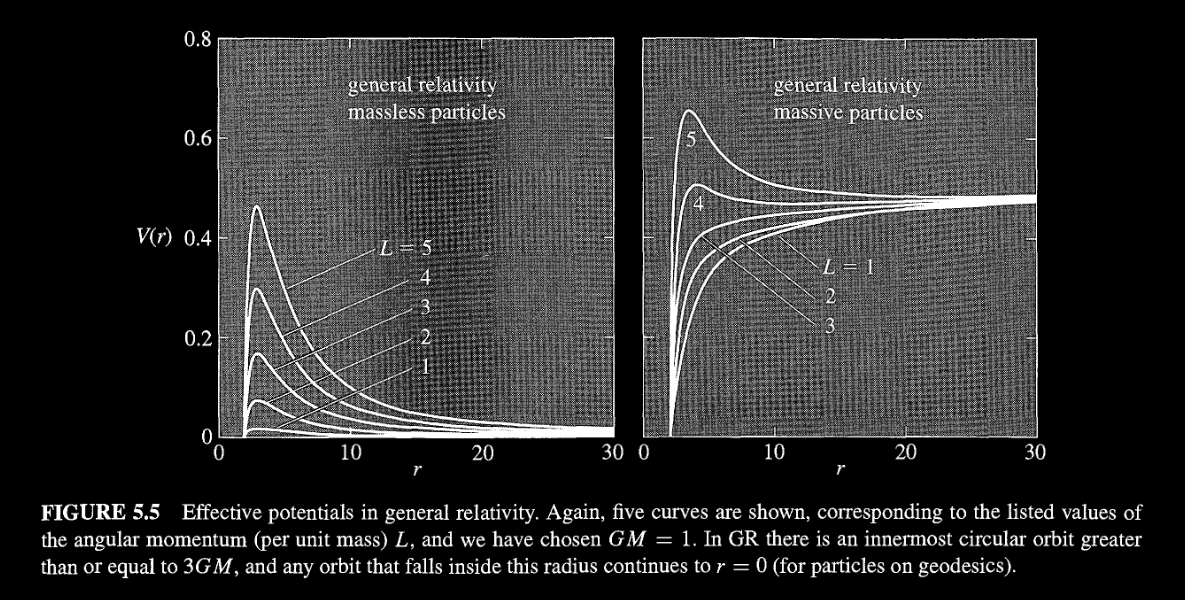
\includegraphics[width=\linewidth]{imm/ex14.png}
\caption{From Carroll}

\label{imm:ex14.png}
\end{figure}

So as always, write down metric, conserved quantities, choose the adequate four-velocity normalization (=0), unravel the tensor product, substitute quantities, get yourself to equation of kinetic radial energy + $V_{eff}\left( r \right) = $ energy of the system. Take $ \frac{d V_{eff\left( r \right)}}{d r}$,  insert values, find stationary point. Should be $r = 3$, again radius of the photon sphere, not just any radius. Go back to equation of conservation of energy and substitute values, you find value of \emph{E}, should be $E = \frac{10}{3\sqrt{3}}$.

\subsubsection{Ex 15}

You apply the gauge transformation to $V_{\mu }$:
\begin{align*}
	V_{\mu } \to  \tilde{V}_{\mu } &= \partial_{\nu }\tilde{h}^{\nu }_{\mu } - \frac{1}{2}\partial_{\mu }\tilde{h}^{\nu }_{\nu } =\\
				       &= \partial_{\nu }\left( h^{\nu }_{\mu } + \partial^{\nu }\xi _{\mu } + \partial_{\mu }\xi ^{\nu } \right) - \frac{1}{2}\partial_{\mu }\left( h + \partial_{\nu }\xi ^{\nu }+\partial^{\nu }\xi _{\nu } \right) = \\
				       &= \partial_{\nu }\left( h^{\nu }_{\mu } + \partial^{\nu }\xi _{\mu } + \partial_{\mu }\xi ^{\nu } \right) - \frac{1}{2}\partial_{\mu }\left( h + 2\partial_{\nu }\xi ^{\nu } \right) = \\
				       &= \partial_{\nu }h^{\nu }_{\mu } + \partial_{\nu }\partial^{\nu }\xi _{\mu } - \frac{1}{2} \partial_{\mu }h + \partial_{\nu }\partial_{\mu }\xi ^{\nu }- \frac{1}{2}2 \partial_{\mu }\partial_{\nu }\xi ^{\nu } = \\
				       &= \partial_{\nu }h^{\nu}_{\mu } + \Box \xi _{\mu } - \frac{1}{2}\partial_{\mu }h
\end{align*}

So this is how the vector changes.\par
I can make $\tilde{V}^{\mu }$ vanish if I choose a gauge such that $\Box \xi _{\nu } = -\partial_{\nu }h^{\nu }_{\mu } + \frac{1}{2}\partial_{\mu  }h$

\subsubsection{Ex 16}
First request: $K^{\mu } = \left( \omega , 0,0,k \right)$, since it propagates along $z^{+}$-axis. Wave vector is light-like
\[
k_{\mu }k^{\mu } = \eta _{\mu \nu } k^{\mu }k^{\nu } = 0 = -\omega ^{2} + k^{2} \to  \omega = \pm k
\]
we used Minkowski metric tensor because we are in linearized gravity. We choose $\omega  = + k$, since it propagates along positive direction of \emph{z-}axis.\par

Second request: C is made of constants, is traceless and $C_{00} = C_{i0} = 0$ and the wave vector is orthogonal to $C_{\mu \nu } \to  k^{\mu }C_{\mu \nu } = 0$. this means
\[
C_{\mu \nu } = \begin{pmatrix}
0 & 0 & 0 & 0 \\
0 & C_{11} & C_{12} & 0 \\
0 & C_{21} & C_{22} & 0 \\
0 & 0 & 0 & 0
\end{pmatrix}  = \begin{pmatrix}
0 & 0 & 0 & 0 \\
0 & C_{11} & 0 & 0 \\
0 & 0 & -C_{11} & 0 \\
0 & 0 & 0 & 0
\end{pmatrix} 
\]
Since we have just $h_{+}$ polarization.\par
About the exponential, $k_{\mu }x_{\mu } = -\omega t + \omega z$, and using Euler's formula $e^{ix} = \text{cos}x + i \text{sin}x$, we get
\[
h^{TT}_{\mu \nu } = \begin{pmatrix}
0 & 0 & 0 & 0 \\
0 & C & 0 & 0 \\
0 & 0 & C & 0 \\
0 & 0 & 0 & 0
\end{pmatrix} \text{cos}\left( \omega \left( z-t \right) \right)	
\]
Third request: we do gauge transformation $h_{\mu \nu }^{TT} \to  \tilde{h}_{\mu \nu }^{TT} = h_{\mu \nu }^{TT} +\partial_{\mu }\xi _{\nu }+\partial_{\nu }\xi _{\mu }$.
We lower index of $\xi ^{\mu } = \left( \alpha \left( x^{\mu } \right), \beta \left( x^{\mu } \right), 0,0 \right) \to  \eta ^{\mu \nu }\xi ^{\nu } = \xi _{\mu } = \left( -\alpha ,\beta ,0,0 \right)$. \par
Now you need to compute the transformation. Since $\tilde{h}^{TT}_{\mu \nu } = h^{TT}_{\mu \nu } + \delta h^{TT}_{\mu \nu } $, with $\delta H^{TT}_{\mu \nu } = \partial_{\mu }\xi _{\nu} +\partial_{\nu }\xi _{\mu }$, we will compute just that. It's not difficult, you know that we have non-zero just $\xi _{0} =- \alpha , \xi _{1}=\beta $, and all $\partial_{\mu }$ are valid.
\begin{equation}
\delta h^{TT}_{\mu \nu } = \begin{pmatrix}
2\partial_{0}\xi _{0} & \partial_{0}\xi _{1}+\partial_{1\xi _{0}} & \partial_{2}\xi _{0} & \partial_{3}\xi _{0} \\
=_{01} & 2\partial_{1}\xi _{1} & \partial_{2}\xi _{1} & \partial_{3}\xi _{1} \\
=_{02} & =_{12} & 0 & 0 \\
=_{03} & =_{13} & 0 & 0
\end{pmatrix}  = \begin{pmatrix}
-2\partial_{0}\alpha  & \partial_{0}\beta -\partial_{1}\alpha  & -\partial_{2} \alpha   & -\partial_{3}\alpha  \\
=_{01} & 2\partial_{1}\beta  & \partial_{2}\beta  & \partial_{3}\beta  \\
=_{02} & =_{12} & 0 & 0 \\
=_{03} & =_{12} & 0 & 0
\end{pmatrix} 
\end{equation}
And then you get 
\[
\tilde{h}^{TT}_{\mu \nu } =\left( h^{TT}_{\mu \nu } + \delta h^{TT}_{\mu \nu }\right) \text{cos}\left( \omega \left( z-t \right) \right)	
\]
Done. 

\subsubsection{Ex 17}

First request: since the wave vector is light-like $k_{\mu }k^{\mu } = 0$, since we are in linearized gravity we will use the Minkowski metric tensor to pull down the index, so
\[
\eta _{\mu \nu }k^{\mu }k^{\nu } = - \omega ^{2} + 2k^{2} \to k = \frac{\omega }{\sqrt{2}} \to  k^{\mu } = \left( \omega , 0, \frac{\omega }{\sqrt{2}}, \frac{\omega }{\sqrt{2}} \right)
\]
Second request: One need to find the rotation matrix, because the requested transformation is a rotation along \emph{x-axis} of $45°$. so 
\[
R^{i }_{j} = \begin{pmatrix}
1 & 0 & 0 \\
0 & \text{cos}45 & -\text{sin}45 \\
0 & \text{sin}45 & \text{cos}45
\end{pmatrix} \to  R^{\mu }_{\nu } = \begin{pmatrix}
1 & 0 & 0 & 0 \\
0 & 1 & 0 & 0 \\
0 & 0 & \frac{1}{\sqrt{2}} & -\frac{1}{\sqrt{2}} \\
0 & 0 & \frac{1}{\sqrt{2}} & \frac{1}{\sqrt{2}}
\end{pmatrix} 
\]
Now $C_{\mu ^{\prime }\nu ^{\prime }}$ is a superposition of superposition of a “+ polarization” with amplitude $h^{\prime }_{+}$  and a “ $\times$ polarization” with amplitude $h^{\prime }_{\times}$ so will be
\[
c_{\mu ^{\prime }\nu ^{\prime }} = \begin{pmatrix}
0 & 0 & 0 & 0 \\
0 & h^{\prime }_{+} & h^{\prime }_{\times} & 0 \\
0 & h^{\prime }_{\times} & -h^{\prime }_{+} & 0 \\
0 & 0 & 0 & 0
\end{pmatrix} 
\]
We want to bring it back to our original system $\left( x,y,z \right)$, and it is possible to use the rule to transform a tensor
\[
C_{\mu \nu } = \Lambda ^{\alpha }_{\mu }\Lambda ^{\beta }_{\nu }C_{\alpha \beta }
\]
But it is far easier and more efficient to use
\[
C = R^{T}C^{\prime }R
\]
and also equivalent. 

What you obtain is
\[
C_{\mu \nu } = \frac{1}{2} \begin{pmatrix}
0 & 0 & 0 & 0 \\
0 & 2h^{\prime }_{+} & \frac{2}{\sqrt{2}}h^{\prime }_{\times} & - \frac{2}{\sqrt{2}}h^{\prime }_{\times} \\
0 & =C_{12} & -h^{\prime }_{+} & h^{\prime }_{+} \\
0 & =C_{13} & =C_{23} & -h_{+}
\end{pmatrix} 
\]


\subsubsection{Ex 18}
Derive by time
\begin{align*}
	\frac{\partial }{\partial t}  H^{2} &= \frac{\partial }{\partial t}  \frac{8\pi G \rho }{3} - \frac{\partial }{\partial t}  \frac{k}{a^{2}}\\
2 \dot{H}H &= \frac{8\pi G \dot{\rho }}{3} - \left( -2\dot{a} \right)a^{-3}k\\
 2\dot{H}H &= \frac{8\pi G}{3}\left( -3H\left( \rho +p \right) \right) + \frac{2k}{a^{2}}H\\
 \text{ simplify H }
 2\dot{H} &= -8 \pi G \left( \rho +p \right) + 2 \frac{k}{a^{2}}\\
 \text{ explicit } \dot{H}, H = \frac{\dot{a}}{a}, \dot{H} = \frac{\ddot{a}a - \dot{a}^{2}}{a^{2}}\\
 2 \frac{\ddot{a}}{a} - 2 \left( \frac{\dot{a}}{a} \right)^{2} - \frac{2k}{a^{2}} &= -8\pi G\left( \rho +p \right)\\
 \text{ put eq.  } H^{2} = \ldots 
 \frac{\ddot{a}}{a} - \frac{8\pi G\rho }{3}+ \frac{k}{a^{2}} &= -4\pi G\left( \rho +p \right)\\
 \frac{\ddot{a}}{a} &= -4\pi G \left( \rho +p-\frac{2}{3}\rho  \right)\\
		    &= \frac{-4\pi G}{3}\left( \rho +3p \right)
\end{align*}
Done

\subsubsection{Ex 19}

Remember $p = w\rho  \to  p = \frac{2}{3}\rho $. \par
First question: $\rho \left( a \right)\propto a $:
\begin{gather*}
\dot{\rho } + 3H\left( 1+w \right)\rho = \dot{\rho }+ 3H\left( \frac{5}{3} \right)\rho  \\
\text{ take directly the solution }\\
\rho \left( a \right) = \rho \left( a_{0} \right)\left( \frac{a_{0}}{a} \right)^{3 \cdot \frac{5}{3}} = \rho _{0} \left( \frac{1}{a} \right)^{5} = \rho _{0}a^{-5}\\
\to \rho\left( a \right)\propto a^{-5}
\end{gather*}
Second question: $a\left( t \right)\propto t$?\par
\begin{gather*}
	\left( \frac{\dot{a}}{a} \right)^{2} = \frac{8\pi G}{3}\rho  - \frac{\kappa }{a^{2}}= C \rho  \\
	\frac{\dot{a}}{a} = \sqrt{C}\rho ^{\frac{1}{2}} = \sqrt{C} \rho _{0} a^{-5/2}\\
	\dot{a} = \sqrt{C}\rho _{0} a^{-\frac{3}{2}} \\
	\frac{d a}{d t} = D a^{-3/2}\\
	\int_{0}^{a}{a^{\frac{3}{2}}da} = \int_{0}^{t}{ D dt}\\
	\frac{2}{5}a^{\frac{5}{2}} = D t\\
	a = \left( \frac{5}{2}D t \right)^{\frac{2}{5}}\\
	a\left( t \right)\propto t^{\frac{2}{5}}
\end{gather*}
Third question: $H\left( t \right)\propto t?$\par
Since $\ddot{a} = \frac{d }{d t} \dot{a}$, then $ \frac{\ddot{a}}{a} = \frac{d }{d t} H$
\begin{gather*}
\frac{d }{d t} H = - \frac{4\pi G}{3} \left( \rho  + \frac{2}{3}\rho  \right) = - C \left( \frac{5}{3} \rho  \right) = - D \rho  \\
dH = - D \rho dt
\end{gather*}
with 
\begin{gather*}
\begin{cases}
\rho  \propto a^{-5} \\
a \propto t^{\frac{2}{5}}
\end{cases} \to \rho \propto t^{-2} \\
\int_{}^{}{dH} = \int_{}^{}{- D t^{-2} dt}\\
H \propto t^{-1}
\end{gather*}
Fourth question: $\rho \left( t \right) \propto t$?\par
Already answered: $\rho \propto t^{-2}$

\subsubsection{Ex 20}


First request: Non relativistic matter has : $\rho \left( a \right) = \rho _{0}a^{-3}$. You need to remember that $\rho _{cr} = \frac{3H^{2}}{8\pi G}$. Write down
\[
\Omega _{M}\left( a \right) = \frac{\rho _{0}a^{-3}}{ \frac{3H^{2}}{8\pi G}} = \frac{8\pi G}{3H^{2}}\rho _{0}a^{-3} \frac{H_{0}^{2}}{H_{0}^{2}} = \Omega _{0} \frac{H_{0}^{2}}{H^{2}}a^{-3}
\]
so remember that 
\[
\Omega _{0} = \frac{8\pi G}{3 H_{0}^{2}} \rho _{0}
\]
Then you write down the Friedmann equation with also Cosmological constant
\[
H^{2} = \frac{8\pi G}{3}\rho + \frac{\Lambda }{3} = \frac{8\pi G}{3}\rho _{0}a^{-3} + \frac{\Lambda }{3}	
\]
Make it to \emph{today}'s values:
\[
H_{0}^{2} = \frac{8\pi G}{3H^{2}_{0}}\rho _{0}H_{0}^{2} + \frac{\Lambda }{3}
\]
After a little manipulation $ \frac{\Lambda }{3} = H_{0}^{2}\left( 1 - \Omega _{0} \right)$, and you put this back in Friedmann Equation to find $H^{2}$, so you can substitute it in $\Omega _{M}\left( a \right)$ equation.\par

Second request: From \emph{acceleration equation}
\[
\frac{\ddot{a}}{a} = - \frac{4\pi G}{3}\left( \rho + 3p \right) + \frac{\Lambda }{3}
\]
since $\rho = \rho _{M}+ \rho _{\Lambda }$ and $p = p_{M} + p_{\Lambda }$, from $p = w \rho $ with $w_{M} = 0, w_{\Lambda } =- 1$, you get
\[
\frac{\ddot{a}}{a} = - \frac{4\pi G}{3} \left( \rho _{M} -2\rho _{\Lambda } \right)
\]
with $\rho _{m }= \rho _{0}a^{-3}$ and
\[
\rho  _{\Lambda } = \frac{\Lambda }{8\pi G} = \frac{3H_{0}^{2} \left( 1-\Omega _{0} \right)}{8\pi G}
\]
You also get that if you want acceleration you need $\left( \rho _{M} - 2\rho _{\Lambda } \right)<0$. Look at $\rho _{\Lambda }$ and see that $\rho _{\Lambda } = \frac{\rho _{0}}{\Omega _{0}}\left( 1-\Omega _{0} \right)$. You put this in the disequation, solve for \emph{a}, put $\Omega _{0} $ value.














